\documentclass[11pt,a4paper]{article}
%\documentclass[conference]{IEEEtran}
\usepackage[english]{babel} 
\usepackage[T1]{fontenc}
\usepackage{lmodern}
\usepackage[utf8]{inputenc}
\usepackage{eurosym}
\DeclareUnicodeCharacter{20AC}{\euro}
\usepackage{graphicx}
\usepackage{rotating} 
\usepackage{array}
\usepackage{booktabs} 
\usepackage{longtable}
\usepackage{ifthen}
\usepackage{xcolor}
\usepackage{tabu}
\usepackage{colortbl}
\usepackage{calc}
\usepackage{pifont}
\usepackage{forloop}
\usepackage[nomessages]{fp}
\usepackage[autostyle]{csquotes}  
\usepackage{amsmath}
\usepackage{amssymb}
\usepackage{amsthm} 
\usepackage{listings}
\usepackage{color}


\newtheoremstyle{break}
   {\topsep}{\topsep}%
   {\itshape}{}%
   {\bfseries}{}%
   {\newline}
   {\thmname{#1}\thmnumber{\@ifnotempty{#1}{ }\@upn{#2}}%
    \thmnote{ {\bfseries(#3)}}}% 
    
\newtheorem{definition}{Definition}

\usepackage[parfill]{parskip}
%\usepackage[onehalfspacing]{setspace}
\usepackage{newclude}

\newcounter{starnumber}
\newcommand{\stars}[1]{
  \forloop{starnumber}{1}{\value{starnumber} < 6}{
    \ifthenelse{#1 < \value{starnumber}}{\ding{73}}{\ding{72}}%
  }
}

\definecolor{mygreen}{rgb}{0,0.6,0}
\definecolor{mygray}{rgb}{0.5,0.5,0.5}
\definecolor{mymauve}{rgb}{0.58,0,0.82}

\lstset{ %
  backgroundcolor=\color{white},   % choose the background color; you must add \usepackage{color} or \usepackage{xcolor}
  basicstyle=\footnotesize,        % the size of the fonts that are used for the code
  breakatwhitespace=false,         % sets if automatic breaks should only happen at whitespace
  breaklines=true,                 % sets automatic line breaking
  captionpos=b,                    % sets the caption-position to bottom
  commentstyle=\color{mygreen},    % comment style
  deletekeywords={...},            % if you want to delete keywords from the given language
  escapeinside={\%*}{*)},          % if you want to add LaTeX within your code
  extendedchars=true,              % lets you use non-ASCII characters; for 8-bits encodings only, does not work with UTF-8
  frame=single,                    % adds a frame around the code
  keepspaces=true,                 % keeps spaces in text, useful for keeping indentation of code (possibly needs columns=flexible)
  keywordstyle=\color{blue},       % keyword style
  language=Octave,                 % the language of the code
  morekeywords={*,...},            % if you want to add more keywords to the set
  numbers=left,                    % where to put the line-numbers; possible values are (none, left, right)
  numbersep=5pt,                   % how far the line-numbers are from the code
  numberstyle=\tiny\color{mygray}, % the style that is used for the line-numbers
  rulecolor=\color{black},         % if not set, the frame-color may be changed on line-breaks within not-black text (e.g. comments (green here))
  showspaces=false,                % show spaces everywhere adding particular underscores; it overrides 'showstringspaces'
  showstringspaces=false,          % underline spaces within strings only
  showtabs=false,                  % show tabs within strings adding particular underscores
  stepnumber=1,                    % the step between two line-numbers. If it's 1, each line will be numbered
  stringstyle=\color{mymauve},     % string literal style
  tabsize=2,                       % sets default tabsize to 2 spaces
  title=\lstname                   % show the filename of files included with \lstinputlisting; also try caption instead of title
}

\renewcommand{\arraystretch}{1.2}

%\usepackage[sortcites=true, style=authoryear,natbib=true]{biblatex}
\usepackage{biblatex}
\bibliography{bibliography}

%Autornamen in Bibliography fett
%\AtBeginBibliography{\renewcommand*{\mkbibnamelast }[1]{\textbf{#1}}}
%\AtBeginBibliography{\renewcommand*{\mkbibnamefirst }[1]{\textbf{#1}}}

%\makeindex

\title{Introduction to Genetic Algorithms}
\date{\today}
\author{Jan-Christoph Klie, Jana-Kira Schomber, Sebastian Muszytowski \\Baden-Wuerttemberg Cooperative State University Mannheim }

\begin{document}

\maketitle
%\twocolumn[
%       \maketitle
%        \begin{@twocolumnfalse}
%        \maketitle
%        \end{@twocolumnfalse}
%]


\section{Introduction}

The general idea of genetic algorithms is based on Darwin's evolution theory, commonly known as "survival of the fittest". In his book "On the Origin of Species" Darwin postulates, that the evolution of species is based on random genetic mutations. The mutation of a single member then results in it being more suited for survival in a certain environment, thus having a higher chance of survival than other, unmutated or differently mutated members of the same species. Subsequently, if the mutated member of the species survives, it is able to reproduce, thus bequeathing its mutated genes to the next generation. This next generation may once again experience random mutations, making the selection repeat itself over and over again.\cite{0691026157} Since this is a process that ideally happens in nature, without any interference from outer sources, this evolution theory is also said to be based on natural selection.

It is common for technique to take nature as a model for how to accomplish certain tasks. In 1975, John Holland was one of the the first ones to suggest using the idea of natural selection to solve complex problems. \cite{9783540731894} The "complex problems" which Holland suggests solutions for are so-called optimization problems. These problems have many possible solutions, however some of them are more optimal than others in regard to a certain goal that is to be attained. A seemingly still simple example of an optimization problem is the problem known as "knapsack problem". 

\begin{figure}[h!]
  \centering
  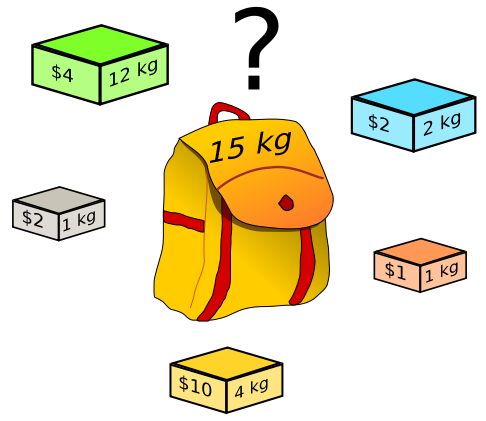
\includegraphics[width=0.5\textwidth]{ks.png}
  \caption{Knapsack Problem Visualisation (from http://www.zhihua-lai.com/wp-images/acm/2012/ks.png)}
  \label{ks}
\end{figure}

The idea is that you have a knapsack which can carry a certain weight. Furthermore you have a number of items, with each item having two distinct attributes: Its weight and its monetary value. The goal is to pack the combination of items in your knapsack that has the highest possible value, taking the weight restriction of the knapsack itself into account.

There are obviously multiple options, and while there is one that is the optimal, meaning the one that wields the highest amount of money, every other combination, while not optimal is also not wrong.

Now if you want to map the principle of evolution on the principle of genetic algorithms, you simply have to get the terminology straight. Simplified, evolution is nothing else but an optimization problem. The goal of an individual is survival. However, while to survive one day and to survive for one year both mean survival, it is obvious that surviving for one year is preferable, thus being the more “optimal”. However in regard to Darwinism it is not as simple as that. While “survival of the fittest” implies that survival is indeed the goal, upon looking closer at the evolution theory that survival alone is not really what makes an individual successful in regard to evolution. Evolution rather is about the passing on of mutated, superior genes. Summed up it is less about the survival of the individual and rather about the survival of the genes of said individual.

Therefore it would be more appropriate to state the goal of evolution as “to have as many individuals inherit the genes as possible”. Otherwise no real change in the whole race of the individual would be possible.

Nonetheless, the accurate formulation of the goal is subsidiary, as it is much more important to note that it is possible to name a goal at all that can be considered as the goal of an optimization problem.

The second part, the parts that make up the solution of an optimization problem are the complete set of genes that make up an individual. If the combination of these genes is beneficial to the goal, an individual is able to live long enough to bequeath its genes to the next generation, possibly even multiple times. However the restrictions of nature have to be taken into consideration. Since each individual already inherits a certain gene pool to begin with, the whole set of its genes would not differ from the one of its parents drastically. 
That is the third, final and most important aspect of and the one that leads to what genetic algorithms are all about. The whole set of genes is changed to a certain degree by mutation of a single or multiple genes. How much mutation is possible in nature is not in the scope of this paper, thus at this point it is sufficient to generalize it with saying that a certain amount of mutation is specified as the limit of possible mutation by nature. The “amount of mutation” means that the mutated gene has to share a certain percentage of characteristics with the original gene.

In a way, this mutation is the natures concept for solving the optimization problem with the goal “to have as many individuals inherit the genes as possible”. Therefore one can now derive the principle after which genetic algorithms function. In general, genetic algorithms start with a starting population. A population is made up of many different combinations of certain features, just like a living being is made up of many different genes. Then the population members are measured for their “fitness” according to how close they are to the stated goal. The fittest members, meaning the ones the closest to the goal are then taken to create a new population, on which the process repeats itself again and again, analogously to the way evolution works according to Darwin’s theory.

After getting a basic understanding of what genetic algorithms are about it might be important to take a look at why genetic algorithms are even needed, before getting into deeper detail about how they even work.
For a better vividness it is usually helpful to take the help of an example on which to base ones assertions. Therefore the already briefly explained knapsack problem will be taken into consideration.
If one takes the problem with the exemplary values from the knapsack problem visualization one has the following scenario:
The knapsack one has available has a limit of 15kg. Therefore one can only pack goods that add up to 15kg or less.
The goods available are the five with the following values:

\begin{table}[h!]
\centering
\begin{tabular}{p{0.3\textwidth}p{0.2\textwidth}p{0.2\textwidth}}
\toprule
    & Weight (kg) & Value (\$) \\
\midrule
Good 1  &  12 &   4\\
Good 2  &  1  &  2\\
Good 3  &  2  &  2\\
Good 4  &  1  &  1\\
Good 5  &  4  &  10\\
\bottomrule
\end{tabular}
\caption{Knapsack item table listing weight in kg and value in dollar.}
\label{tbl:ks_prob}
\end{table}

Since their weight adds up to a total of 20kg it is obviously impossible to carry all of them with a knapsack that can only carry 15kg. Thus one has to make a decision what is to be taken and what is to be left behind.
The possible solutions are made up of the combinations of the items with the goal of having the maximal value.
As a human, this sort of intellectual game is fairly easy to solve for the given conditions. Intuitively one would immediately pack Good 5, since it has the highest value with 10\$ but only weighs 4kg. Afterwards, the next good to consider would be the Good 1 with second highest value. However its weight is 12kg, meaning it would add up to 16kg together with the 4kg heavy Good 5, ruling out the possibility of combining the both of them since they would break the limits given by the knapsack.
Afterwards one simply has to take a look at the weight of the remaining goods to notice that Good 2-4 have a total weight of 4kg, hence making it possible to take all of them together with Good 5. The final value of the Goods in the knapsack is 15\$, while still only weighing 8kg.

Obviously there are other combinations, like taking Good 1, 2 and 3, which would result in a value of 8\$, or taking Good 1, 2, and 4, resulting in 7\$. However, no matter which other combination you choose, you will never exceed 15\$.
This is logical, as Good 5 with its value of 10\$ is essential. Even if one adds up the value of all remaining goods the result is only 9\$. Furthermore Good 1 and Good 5 are mutually exclusive, which means that only one of both can be taken. The case is pretty clear with the given values.

However the situation already changes when the disparity of the weight and value of all the goods is not as big as with the given ones, because then the choice would not be that obvious. Nonetheless the solution would still be fairly easy to solve since there are only a total of $2^5=32$ possible solutions, since the order in which the goods are packed into the knapsack are of no importance. It might be a hassle, but it is still possible to try out all 32 solutions by hand if one has no other concept by which to work.
However the number of possible solutions expands exponentially depending on how many goods you have available. With one more good the number possible solutions already equals 64 and with doubling the number of goods 1024 solutions are possible. If the chosen weight and value of the goods are still chosen with as much disparity as they were in the example a human might still be able to solve the knapsack problem with ten goods almost as easily as with five.
Nonetheless it is difficult to name a real algorithm for the optimization that works every time and does not rely on trying out every possible solution and checking them for optimality and being in check with the limitations. A computer therefore would generally result to the latter method of calculating every solution.

While calculation power seems to be growing very fast nowadays, the exponential growth of necessary calculations with optimization and combination problems results in a problem being out of calculability for a computer.
This is where the genetic algorithm come into play. For the solution of optimization problems they do not rely on calculating every single combination, as already mentioned beforehand.

Genetic algorithms can all be constructed according to a so-called “cooking recipe”, since they always implement the same steps. One can argue about how many steps there are in total, but for the sake of this paper the number of steps will be broken down to four.
\begin{description}
\item[1. Initialization] \hfill \\ A starting population is created randomly. The total size of the population can be chosen freely. The bigger the population, the higher is the number of possibilities covered and the higher the chance to have a member with an optimal solution. However it has to be taken into consideration that the calculation power and needed storage increases as well.
This step is only executed once.
\item[2. Evaluation] \hfill \\ The next thing is to evaluate each member of the population. The evaluation shows which members are the “fittest”, while the fittest in this context means the closest to the goal.
Furthermore this is the point where a termination condition will be implemented. Since one does start of with the premise of not knowing what value the optimal solution has, one can not simply say once that value is reached the algorithm may stop. Without the termination condition the algorithm would never end, so it is essential to use a termination condition when one does not want to create an infinite loop. There are different possible termination conditions. For example one could say one is satisfied if the fitness value of a member is above or below a certain value. Another option would be to specify a percentage of how many member have to have the same fitness value for the algorithm to stop because apparently there are no more major changes among the population.
\item[3. Creation of the next population] \hfill \\ This step is actually more complex, but all of the following steps can be summarized by the creation of the next population. After all of the substeps are completed, the result is the next population which will then again go through step 2 and 3, so long until the termination condition is met.
\begin{description}
\item[a. Selection] \hfill \\
First of all the members of the population have to be selected which will then be used for step 3.b., namely the Crossover. There are many different methods and algorithms for which members are to be selected, since the selection of the members is the foundation for the next population, as this one will be based on the selected members to a certain degree.
A very simple approach would be to sort the members according to their fitness values and then always take the two most compliant with the goal.
\item[b. Crossover] \hfill \\
As with real genetics, the selected members represent the parents that are combined to create a certain number of offspring. As with the selection there are different methods and algorithms after which the combination can be performed. The goal simply is to generate offspring that inherit traits of both their parents. The idea is, that through the combination of the traits of two “good” members of the population an even “better” member might be created. If one is to take a population of binary numbers, the combination of 11000111 and 10011000 may yield the following offspring: \\

\begin{table}[h!]
\centering
\begin{tabular}{p{0.2\textwidth}p{0.1\textwidth}}
Parent 1  &  1100|0111\\
Parent 2  &  1001|1000\\
Offspring 1 &  1100|1000\\
Offspring 2 &  1001|0111\\
\end{tabular}
\end{table}

For the first offspring the first part of the first parent was combined with the second part of the second parent, while for the second offspring the second part of the first parent was combined with the first part of the second parent.
The combination is denominated with the term “Crossover” in the context of genetic algorithms.
\end{description}
\item[4. Mutation] \hfill \\
The last step in creating a new population is the mutation of the offspring. This is necessary 
\enquote{to prevent falling all solutions in the population into a local optimum of solved problem}\cite{Ezziane:2002:SKP:965702.965705}. The mutation means to modify the offspring a little bit, so that it still has a resemblance with its parents but is slightly different nonetheless.
Taking on the example of binary numbers used for the crossover, one can for example define mutation as flipping one bit of the number, meaning turning either a 1 into a 0 or the other way round. The bit that is to be changed may be selected randomly or according to a certain algorithm.
For example, if the bit at the position seven is chosen for the first offspring, it would turn from the unmutated 11001000 to the mutated 11001010.
\end{description}

In relation to the knapsack problem, the solution with a genetic algorithm according to the cooking recipe is possible.\cite{Ezziane:2002:SKP:965702.965705}
For the calculation base for evaluation a data structure we call good is used that consist of the weight of an item and its value, for example (12|4) would represent Good 1. All of these goods are stored in an array, which will be used for evaluation of the random population.
Afterwards, the initial population is generated. One member of said population is one array the size of the number of goods, where a 1 represents that the good is in the knapsack while 0 means it is not. Each position in the array corresponds with the number of the good. A certain amount of members are created by randomly assigning 0’s and 1’s to various array. After the initial random population is created, each member is evaluated according to its fitness. Therefore the calculation base is taken into account. The fitness value for each member equals the monetary value the member would yield by combination of the items.
There are many different options on how to chose the termination condition, but for the sake of the example it will be that once we have a value of 25\$ in our knapsack we are satisfied. Obviously it is assumed, that the optimal solution is above 25\$, so that our termination condition can be met.

After checking that the initial population does not already meet the termination condition the creation of the next population starts. Various members are selected to be the parents of the offspring that make up the next generation. Uncaring of what algorithm is used for the selection of the parents, the members that are no valid solution for the problem because their weight exceeds the limits are excluded from being selected.

After selection, crossovers are performed on the selected parents just as mutations are performed on the offspring.
By repeating the steps two and three, namely the evaluation of the population and the creation of a new one eventually an array will be produced, that satisfies the termination condition of having a fitness value above 25.
It might seem a little less reliable to use a genetic algorithm, since for one one relies on the principle of randomization to a certain degree to solve the problem and for another there is no guarantee how good the solution the program might yield will be. With every run the program is likely to return a solution that may differ from the solution returned in the previous runs, especially if there are many possible factors, like many different goods with the knapsack problem.
Nonetheless genetic algorithms are, while at first seeming counterintuitive with their randomness, a helpful approach in optimization problems, as they are one approach that actually produces a result and does require comparatively few resources in regard to the calculation of each possible solution. Although one has to be vary that this is only the case given a certain point of complexity the problem at hand.

Certainly, solving the knapsack problem with a genetic algorithm when one only has five given items is an unwise approach, but when faced with 10, 15, 20 or an even bigger number of goods to choose from a genetic algorithm will be able to calculate a possibly optimal solution.

\section{The Traveling Salesman Problem}

The traveling salesman problem is a problem in theoretical computer science aimed to determine the shortest path for a given list of cities. The problem is NP-hard which means that the problem is non deterministic and can be solved in polynomical time. There are many approaches to solve the problem, for instance by generating all possible path combinations and choose the shortest path. As one may expect this naive approach involes a lot of calculations and ressources.

A much more effective way to solve the traveling salesman problem is by applying the principle of genetic algorithms. The solution produced by the genetic algorithm may not be the optimal solution but converges nearer to the optimal solution in each iteration. 

\subsection{Implementation}

The traveling salesman problem can be implemented using genetic algorithms and the principle behind those. For demonstration purposes the genetic algorithm is implemented in the programming language python.

\begin{figure}[h!]
  \centering
  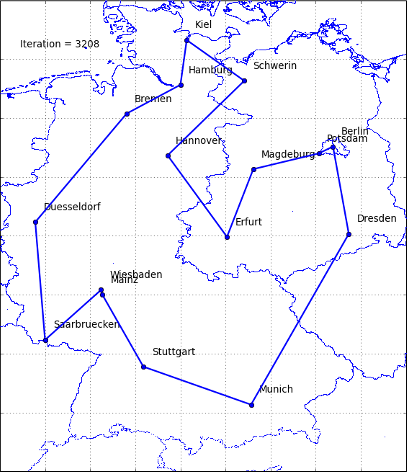
\includegraphics[width=0.5\textwidth]{tsp.png}
  \caption{Screenshot of the genetic traveling salesman program (own work)}
  \label{ks}
\end{figure}


At the beginning there is the initial population where each member of the population represents a potential route. This population is initialized using a cities vector which holds all cities. A permutation function is applied to the cities vector which results in a intitial path.\\
\begin{lstlisting}[language=Python]
population=np.zeros((cities,cities+1))
for j in range(cities):
  population[j,0:cities]=np.random.permutation(cities)
  population[j,cities]=population[j,0]
\end{lstlisting}
After the initial population holds its individual routes, a function to determine the quality of a route is necessary to evaulate the quality of each population member. In the application of the traveling salesman the evaluation function calculates the total distance traveled between all cities with regard to the shape of the world. Therefore the distance between each city is calculated using the following code and then accumulated.\\
\begin{lstlisting}[language=Python]
def distance(origin, destination):
  lat1, lon1 = origin
  lat2, lon2 = destination
  radius = 6371 # km
  dlat = math.radians(lat2-lat1)
  dlon = math.radians(lon2-lon1)
  a = math.sin(dlat/2) * math.sin(dlat/2) + math.cos(math.radians(lat1)) * math.cos(math.radians(lat2)) * math.sin(dlon/2) * math.sin(dlon/2)
  c = 2 * math.atan2(math.sqrt(a), math.sqrt(1-a))
  d = radius * c
  return d
\end{lstlisting}                        
Since calculation of the distance requires a lot of computation and the distance between cities is static, it can be done prior to the execution of the genetic algorithm. Therefore the program contains a storage vector which holds the distance between each of the cities specified in the problem description. 

Similar to the cooking recipe of the generic genetic algorithm description, the problem is implemented. At first the population is created/initialized and then the genetic functions are applied to each generation until the maximum number of generations is reached.
In python like pseudo-code the algorithm works as follows:\newpage
\begin{lstlisting}[language=Python]
# Create Population
initializePopulation()

# Work with Population
while Iteration < MaxGeneration:
  foreach Individual:
    calculateFitness()
  chromosomeSelection()
  chromosomeCrossing()
  chromosomeMutation()
  naturalSelection()
\end{lstlisting}
In each generation iteration the fitness of each individual of the population is calculated using the already introduced accumulation of distances. In the context of genetic algorithms this accumulation function is called fitness function.

After that chromosomes for crossing are selected. Since the algorithm is based on the principle of the survival of the fittest, the individuals with the highest compliance to the goals are chosen. These chosen individuals will then perform the crossover of chromosomes based on the simplest applicable approach: the single point crossover.

The single point crossover is a technique where a crossing point is chosen randomly in the gene sequence. The first child will get the genes up to the crossing point from one parent and the genes from the crossing point up to the end from the other parent. The genes of the second child are constructed by reversing the order of the parents. Other methods for crossing exists and their application may vary depending on the complexity of the problem. 

A reference-implementing of the single point crossover in python follows, assuming that the number of genes in newly generated child always equals the number of genes of the parents:\\
\begin{lstlisting}[language=Python]
if np.random.rand() < crossing:
  cp=np.ceil(np.random.rand()*cities)
  for a in range(0, cp):
    child1[a] = parent2[a]
    child2[a] = parent1[a]
  for a in range(cp, cities):
    child1[a] = parent1[a]
    child2[a] = parent2[a]
\end{lstlisting}

Since crossing always yields children with similar genes (compared to the population), mutation is needed to vary those children a bit. To control mutation behaviour, a mutation probability is needed. In addition to the probability of mutation, a random gene must be chosen for the mutation.

Additional mutation operations such as switching/swapping the first and last gene can be performed to increase the diversity. In the application of the traveling salesman the switch of the last and first gene increases the chance to find a completely new solution. In python the mutation can be realized in the following way:\\

\begin{lstlisting}[language=Python]
if np.random.rand()<mutation:
  mutInd=np.ceil(np.random.rand(2)*(cities-1))
  first=child1[mutInd[0]]
  second=child1[mutInd[1]]
  child1[mutInd[0]]=second
  child1[mutInd[1]]=first
  child1[-1]=child1[0] # last element and first element switch
\end{lstlisting}

Finally the newly created and maybe mutated children must be integrated into the population. Since the population size is fixed the process of natural selection must erase or respectively replace the weakest members of the population. Depending on the fitness of the children, the newly generated children may be erased.

Programmatically the replacement of the weakest members works as follows:\\

\begin{lstlisting}[language=Python]
for index in range(cities,0,-1):
  if sortedCost[index]>costChild1 and not replace1:
    if child1 not in sortedPopulation:
      sortedPopulation[index]=child1
      replace1=True
  elif sortedCost[index]>costChild2 and not replace2:
    if child2 not in sortedPopulation:
      sortedPopulation[index]=child2
      replace2=True
    if replace1 and replace2:
      break
\end{lstlisting}

After the replacement which mimics the natural selection, the whole process described earlier is repeated until the maximum number of generation is reached. At the end of all iterations the fittest member represents a near optimal solution to the problem evaluated. In the case of the traveling salesman on the sixteen capital cities of Germany, about 5000 generations are needed to reach a near optimal solution. Depending on the initital population, mutation probability and crossover probability a value near the optimum is reached in less iterations or, in worse scenario in more iterations.

\nocite{*}
\printbibliography
\addcontentsline{toc}{part}{References}
\end{document}
